\chapter{Reference}
\label{Reference}
\typeout{$Id$}

\section{Main Window}
\label{Main}

\begin{figure}[hbpt] \begin{centering}
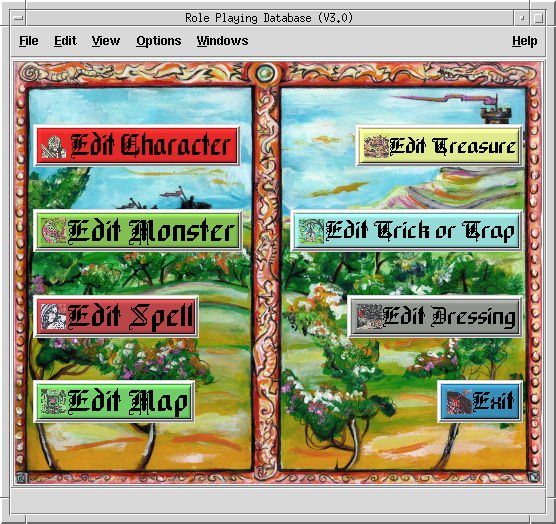
\includegraphics[width=5in]{MainWindow.png} \caption{The main window of
the Role Playing Database} \label{fig:main} \end{centering}
\end{figure} The main window, shown in Figure~\ref{fig:main}, contains
buttons for the seven game informational editors: Character, Monster,
Spell, Treasure, Trick / Trap, Map, and Dressing.  See
Section~\ref{SheetEditor} for a documentation on the Character,
Monster, Spell, Treasure, Trick / Trap, Dressing editor windows and
Section~\ref{Map} for documentation the Map editor window. An eighth
button selects for program exit. In addition to the eight buttons,
there are drop down menus on a menu bar.  The same menu bar is used on
all of the major top level screens.  The File menu has the standard
New, Open, Save, Save As, Print, Close, and Exit menu items, all of
which have the expected meanings and functionality.  The New and Open
menu items on the File menu use cascading menus to select the sort of
thing to create or open.  The Options menu contains menu items to
create/edit (see Section~\ref{sect:configuration}), read, and write the
program's main configuration file, plus a menu item to edit template
files, which opens the ``Sheet Template Editor'' window (See
Section~\ref{Template}), which is used to create and maintain the sheet
editor windows.  The Windows menu contains menu items to select one of
the existing top level windows. The Help menu provides access to the
on line help system (see Chapter~\ref{Help} for complete information
about using the on-line help).

\section{Configuration Editor}
\label{sect:configuration}

\begin{figure}[hbpt]
\begin{centering}
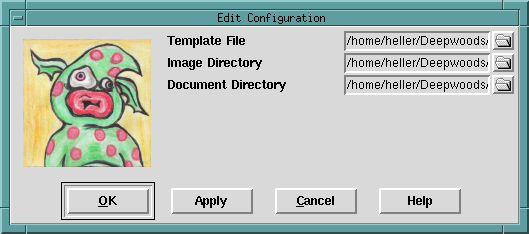
\includegraphics[width=5in]{ConfigurationEditor.png}
\caption{The Configuration Editor Window}
\label{fig:confedit}
\end{centering}
\end{figure}
In Figure~\ref{fig:confedit} is shown the Configuration Editor Window. 
There are three configuration options: the template file to use when
creating new informational sheets, the initial directory to look in for
images for graphic elements, and the initial directory to look in for
external documents.  The configuration file is located in the current
user's home directory in a file named \verb=.roleplayingdb3= under
UNIX/Linux and MacOSX and \verb=roleplayingdb3.rc= under MS-Windows. 
This file is a plain text file containing key, value pairs.  Do not edit
this file by hand though.  Be sure to use the Configuration Editor. 
This makes sure that the file is properly formatted to be read in at
program start time.

\section{Sheet Template Editor Window}
\label{Template}

\begin{figure}[hbpt]
\begin{centering}
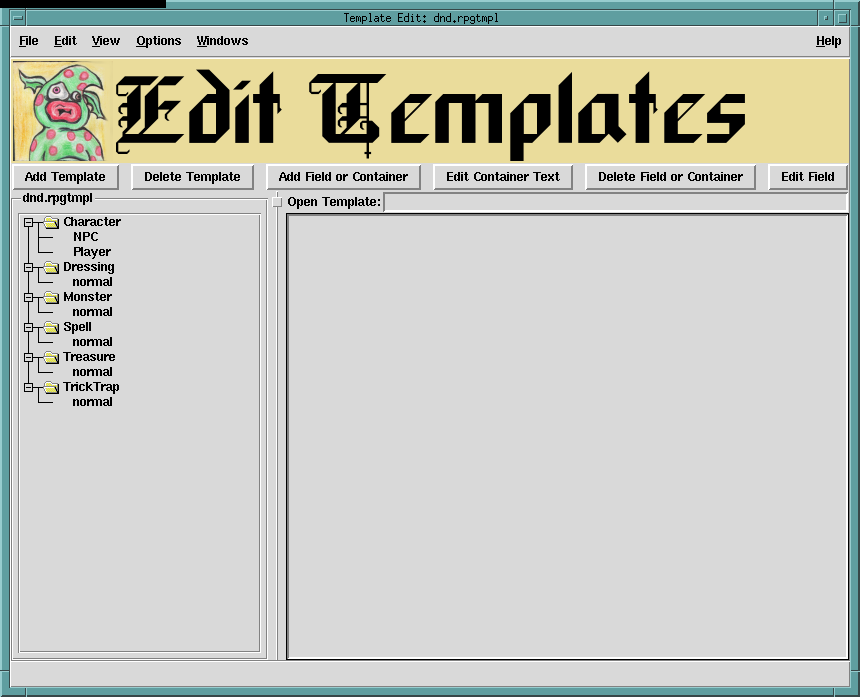
\includegraphics[width=5in]{TemplateEditor1.png}
\caption{The initial Template Editor Window}
\label{fig:tmped1}
\end{centering}
\end{figure}
\begin{figure}[hbpt]
\begin{centering}
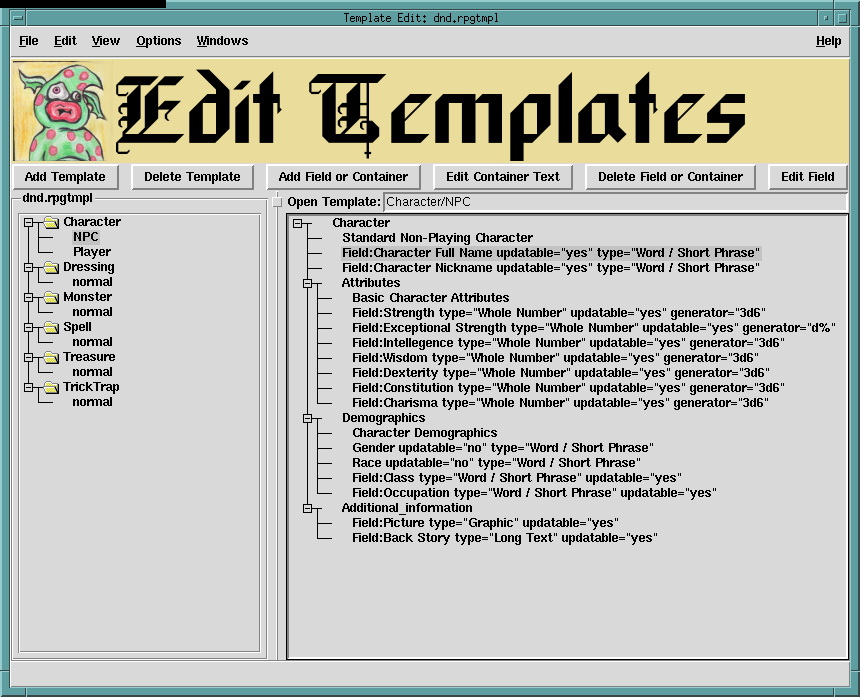
\includegraphics[width=5in]{TemplateEditor2.png}
\caption{The Template Editor Window after loading a template}
\label{fig:tmped2}
\end{centering}
\end{figure}
To allow for differences in game systems, game data elements are
defined with the use of templates.  These templates define what
information is recorded for each game element for a given game system. 
These templates are created and maintained with the template editor. 
The template editor in invoked from the Options menu.  The editor is
shown in Figures~\ref{fig:tmped1} and \ref{fig:tmped2}.  A sheet
contains a top level container which in turn contains zero or more fields
or containers.  Containers can contains zero or more fields or
containers.  Fields and containers have names. Fields also have a type,
possibly a generator (dice combination), and a flag that indicates whether the
field value can be updated.  There are five defined field types:

\index{Field types|(}
\begin{enumerate}
\item \textbf{Whole Number:} This is a numerically valued field. It is either
an arbitrary (usually fixed) value or the result of a dice throw.
\item \textbf{Word / Short Phrase:} This either a single word or a short
(one line at most) phrase, generally describing a textual attribute,
such as a name or some sort of descriptive condition or status.
\item \textbf{Long Text:} This is a multi-line, but short (1-2 paragraph)
text value.
\item \textbf{Graphic:} This is a picture file.  Most standard graphics
formats are supported, including GIF, PNG, JPEG, BMP, TIFF, TGA,
PostScript, and Sun Raster.  The graphic file will be displayed in the
sheet editor window.
\item \textbf{Document:} This a document file.  Any sort of external file
is supported.  The external file will be copied into the sheet file. 
The sheet editor will not attempt to display or otherwise process the
file, but since the file will be ``carried'' along with the sheet file,
it will be available and extractable as needed.
\end{enumerate}
\index{Field types|)}

The generator attribute is only used for numerically valued fields and
the updatable attribute can only be set to no for the word / short
phrase and numerically valued fields.

The templates are used for Character, Monster, Spell, Treasure, Trick /
Trap, and Dressing sheet editors.  The Map editor uses a set of hard-coded
templates. These templates define the fields, their attributes, and
grouping / organizational structure.  Containers have a text attribute
that is used as a section heading for the group of fields contained in
the container. The included template file, \verb=dnd.rpgtmpl=, defines
informational sheets suitable for \textit{Advanced Dungeons and
Dragons}, but template files for other game systems can be created.

The template editor lists the defined templates in the open template
bundle in its left side bar and the currently open template is
displayed in its main display area.  It has a six button tool bar.
Except for the \verb=Add Template= tool bar button, these buttons work
with the current selected or hightlighted item.  An item (template,
container, or field) is selected with a single click of the mouse
button\footnote{Normally the left button.}.


\begin{enumerate}
\item \textbf{Add Template:} A new template is added with the 
\verb=Add Template= tool bar button.  A dialog box prompts for the name
and class of the new template.  The class of the template defines the
outermost container name (same as the class name) and the folder in the
template bundle where the template resides. 
\item \textbf{Delete Template:} An existing template is deleted by
highlighting the template name in the template list and then clicking
the \verb=Delete Template= tool bar button.  A confirmation dialog box
confirms the removal of the template. 
\item \textbf{Add Field or Container:} A field or container is added to
an existing container by highlighting the parent container and clicking
the \verb=Add Field or Container= tool bar button.  A dialog box is
displayed to define the new field or container's attributes. 
\item \textbf{Edit Container Text:} Each container, including the
outermost, can have one-line or text associated with it.  This text is
used as a header.  Highlighting the container and clicking the
\verb=Edit Container Text= tool bar button allows for editing this text
field. 
\item \textbf{Delete Field or Container:} A field or container is
deleted by highlighting the field or container and then clicking the
\verb=Delete Field or Container= tool bar button.  A confirmation
dialog box confirms the removal of the field or container. Note that
removing a container also removes the fields and containers it
contains. 
\item \textbf{Edit Field:} A field's attributes can be edited with the
\verb=Edit Field= tool bar button.  The field to be edited needs to be
highlighted first.  Field names cannot be changed.
\end{enumerate}

To edit a template double click on the template name.  The template
will be opened up in the template editing window. The editing buttons
can be used to create or edit fields and containers.  It is also
possible to use the right mouse button\footnote{Control with the left
or only button under MacOS.} to pop up edit menus to perform editing
functions, including adding and deleting fields and containers from a
container, editing the container's text, and editing a field's
attributes.

The ordering of fields and containers can be altered by draging fields
or containers with the middle mouse button\footnote{Under MacOSX and
MS-Windows, the left or only button with the Alt key is used.}.  Fields
and containers cannot be moved outside of the main class container.

A template file is a Zip archive file containing directories for each
class of sheet: Character, Monster, Spell, Treasure, Trick / Trap, and
Dressing.  These directories in turn contain the template XML files,
which define the structure of the sheets.  It is possible to have
multiple templates for any given class.  It is also possible to have no
templates for a given class.  Not all game systems have all classes of
these things and others might have several sub-classes, sometimes with
very different attributes.

\section{Sheet Editor Windows}
\label{SheetEditor}

\begin{figure}[hbpt]
\begin{centering}
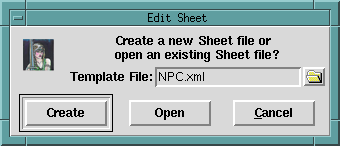
\includegraphics{CreateOrOpenChar.png}
\caption{The Open or Create Character dialog box}
\label{fig:opencreatechar}
\end{centering}
\end{figure}
\begin{figure}[hbpt] 
\begin{centering}
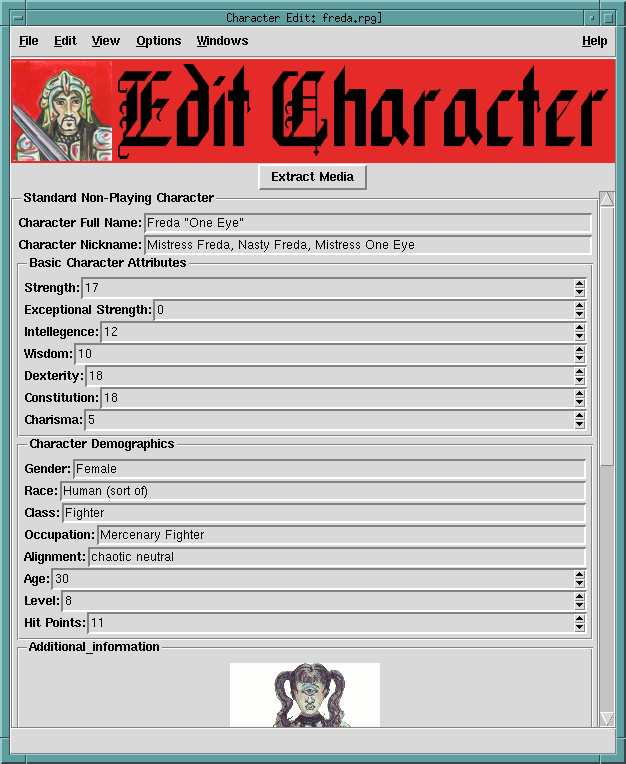
\includegraphics[width=5in]{CharacterEditor.png} 
\caption{The Character Editor window of the Role Playing Database} 
\label{fig:char}
\end{centering} 
\end{figure} 
The Sheet Editor Window, which includes the Character Editor, shown in
Figure~\ref{fig:char}, is used to edit characters, both playing and
non-playing characters, monsters, spells, treasure, tricks / traps, and
dressing items.  It uses one of the sheet templates defined in the
current template file (see Section~\ref{sect:configuration}).  When one
of the sheet editor buttons on the main window are clicked on, a small
dialog box is displayed (shown in Figure~\ref{fig:opencreatechar}),
asking if you want create a new sheet file, using a selected template
or open an existing sheet file. The Monster, Spell, Treasure,  Trick /
Trap, and Dressing Editor Windows are the same as the Character Editor,
but use different templates.

In addition to the fields created from the sheet template, there is also
a tool bar button, labeled ``Extract Media''.  This button allows for the
extraction of embedded media files contained within the sheet file. 
This allows for the use of external editors or viewers with these files.

A sheet file is a Zip archive containing two directories, xml and media.
The xml contains a file named sheet.xml, which is an XML file containing
the sheet information.  The media directory contains any media files
associated with the sheet--this could be pictures or other documents.

\section{Map Editing Windows}
\label{Map}

Map objects are three dimensional, consisting of one or more levels,
above, below, or at ground level.  Each level consists of spaces
(squares or hexagons) arranged on a two dimensional grid.  Each level
is at a depth, where a depth of 0 is ground level, negative depths are
below ground, and positive depths are above ground.  Spaces have an X
and Y coordinate, which are whole numbers ranging between -1000 and
1000, with 0 being the center of the level and -1000 being the extreme
left or western edge (X) and extreme top or northern edge (Y) and 1000
being the extreme right or eastern edge (X) and extreme bottom or
southern edge (Y). Creating or editing a map is a hierarchical process. 
You select the level to create or edit from the main map window
(Figure~\ref{fig:MapEditor}) and you select the space to create or edit
from the level editor window (Figure~\ref{fig:LevelEditor}) for the
level the space is on.  The whole map, with all of its levels and
spaces are stored in a single file, for easy transport and exchange.  It
is possible to have a ``sparse'' map, with levels and/or spaces
omitted.  These might be levels or spaces that have not been
constructed (yet) or are otherwise inaccessible.  With suitable
technology or magic (eg a teleport device or spell) it is possible to
get to non-adjacent spaces or levels.  No attempt it made it enforce
connectivity to adjacent spaces or levels!

There are three map editing windows:
\begin{enumerate}
\item The main map editor, shown in Figure~\ref{fig:MapEditor}, contains
information about the overall map, including the name of the map, the
name of the campaign, and the name of the game master.  This window is
described in Section~\ref{sect:mainmap}.
\item The level editor, shown in Figure~\ref{fig:LevelEditor}, contains
information about a selected level. This window is
described in Section~\ref{sect:leveledit}.
\item The space editor, shown in Figure~\ref{fig:SpaceEditor}, contains
information about a space. This window is
described in Section~\ref{sect:spaceedit}.
\end{enumerate}

\subsection{Main map editing window}
\label{sect:mainmap}

\begin{figure}[hbpt] 
\begin{centering}
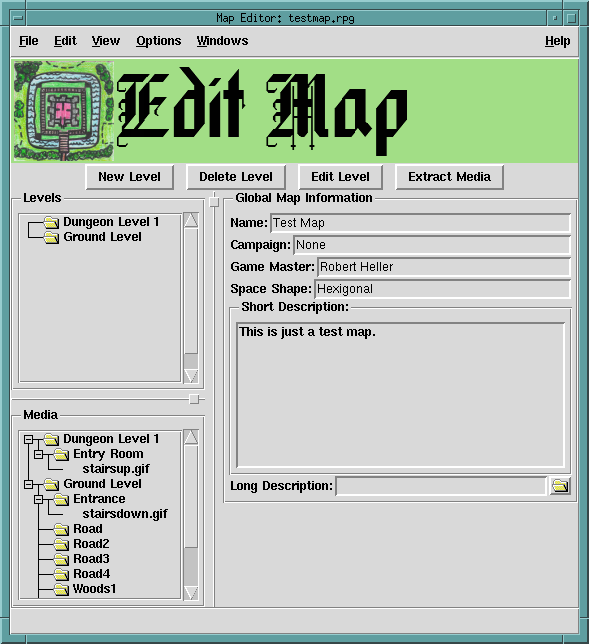
\includegraphics[width=5in]{MapEditor.png}
\caption{Main map editor window}
\label{fig:MapEditor}
\end{centering}
\end{figure}
The main map editor (Figure~\ref{fig:MapEditor}) contains information
about the overall map.  This information includes name of the map, the
name of the campaign, and the name of the game master.  There is space
for a brief description of the map and it is possible to include a
larger document providing a detailed writeup about the map or game
campaign.  Also on this window is a list of levels and a directory tree
of included media.  There is a tool bar with 4 buttons:

\begin{enumerate}
\item New Level--this button creates a new level.
\item Delete Level--this button deletes a selected level.
\item Edit Level--this button edits a selected level.
\item Extract Media--this button extracts a selected media file, making
it available for an external program to view or otherwise process.
\end{enumerate}

\subsection{Level editing window}
\label{sect:leveledit}

\begin{figure}[hbpt] 
\begin{centering}
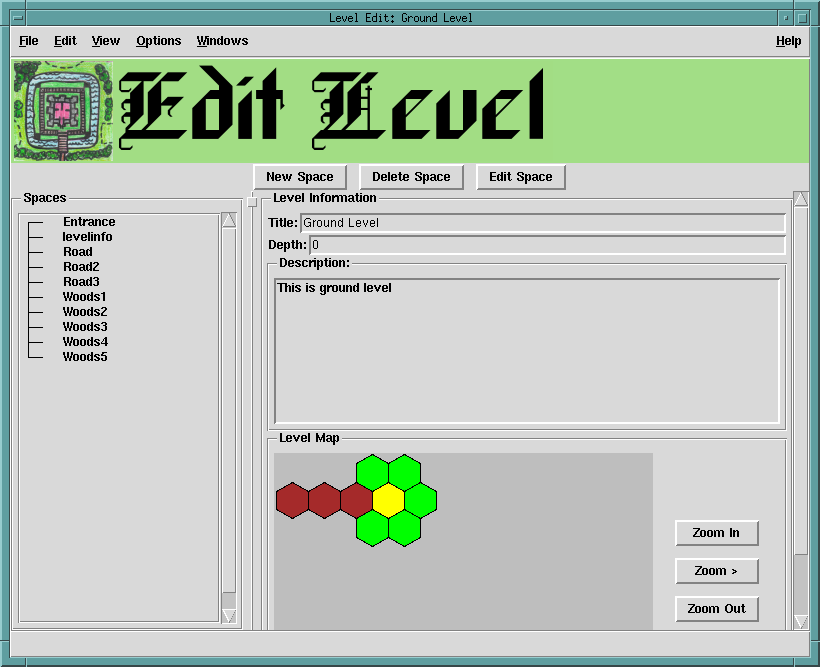
\includegraphics[width=5in]{LevelEditor.png}
\caption{Level editor window}
\label{fig:LevelEditor}
\end{centering}
\end{figure}
The level editor (Figure~\ref{fig:LevelEditor}) contains information
about a selected level.  This information includes the title of the
level and its depth (positive depths are above ground, negative depths are
below ground and a depth of zero is at ground level).  Also included is
a space for a brief description of the level and a map of the level as
well as a list of spaces.

There is a tool bar with three buttons:
\begin{enumerate}
\item New Space--This button creates a new space.
\item Delete Space--This button deletes an existing space.
\item Edit Space--This button edits an existing space.
\end{enumerate}

\subsection{Space editing window}
\label{sect:spaceedit}

\begin{figure}[hbpt] 
\begin{centering}
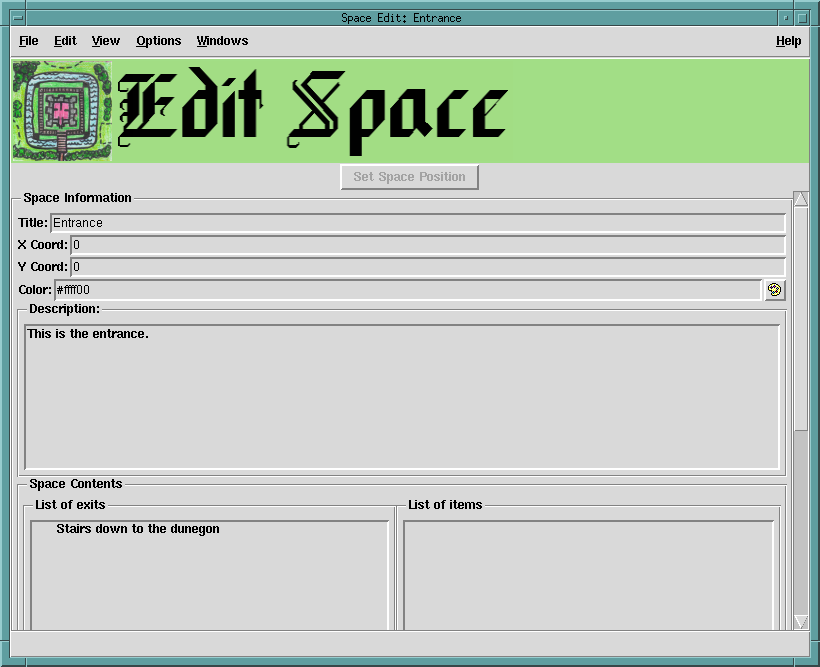
\includegraphics[width=5in]{SpaceEditor.png}
\caption{Space editor window}
\label{fig:SpaceEditor}
\end{centering}
\end{figure}
The space editor (Figure~\ref{fig:SpaceEditor}) contains information
about a selected space.  This information includes the title of the
space, its X and Y coordinates, its color and a short description. 
There is also a pair of lists, one of exits from this space to another
space and a list of other items in the space (such as treasure,
monsters, tricks, traps, and any other odds and ends).  There is also a
map of the space, showing the location of every listed exit or item in
the space.

Below the item and exit lists are triplets of buttons: adding,
deleting, and editing an item or exit.  The main difference between an
item and an exit is that exits have a ``pointer'' to a space and level.
Otherwise, both have a name, a short description, a location within
the space, a graphic, and a sheet file.  The location is an X,Y value,
where the  X and Y values range between -320 and 320, where 0,0 is the
center of the space.  This location is just a relative location within
the space and does not represent any particular distance, other than
that -320 represents the top (Y) or left (X) sides and 320 represents
the bottom (Y) or right (X) side.  The sheet file is optional (this
would make sense if the item or exit was a trick, trap, treasure,
monster, etc.).

When a space is first created, there is available a tool bar button that
can be used to position the space with the mouse.  Once the space has
been saved, its location is fixed and it cannot be moved.  The ``color'' is
arbitrary and is used to color the space on the level map and it is also
used as the space's background color on the space map in the space
editor.  This of course makes it easier to keep track of where spaces
are on the level map.  A game master can use the colors to ``code''
different spaces as having some particular property or feature, such as
coloring wooded areas green and mountainous areas brown and towns with
yellow and castles in blue for example.

\section{Printing}

All main windows have a \verb=Print...= menu item on the \verb=File=
menu. Except for the main window, this menu item allows you to print the
sheet, template, map, level, or space to a PDF file.  At present there
is no support to print directly to your printer, but there are many
programs to print a PDF file to a printer.  A PDF file can also be
shared with someone who does not have the Role Playing Database system
or a PDF file can be uploaded to a website or posted to a blog.  The
\verb=Print...= menu item will ask for the name of the file to be
created.  In the case of the Map and Level editors, you also have the
option of printing the levels (in the case of a Map editor window) or
the spaces (in the case of a Level editor window) or not.
